\section{Definition}

\begin{frame}
	\begin{block}<1->{}
				Ein \textbf{Graph} G besteht aus einer Menge X [deren Elemente Knotenpunkte genannt werden] und einer Menge U, wobei jedem Element u $\in$ U in eindeutiger Weise ein geordnetes oder ungeordnetes Paar von [nicht notwendig verschiedenen] Knotenpunkten, x,y $\in$ X zugeordnet ist.
				Ist jedem u $\in$ U ein geordnetes Paar von Knoten zugeordnet, so heißt der Graph \textbf{gerichtet}, und wir schreiben 
				$G= (X, U)$.
				Die Elemente von U werden in diesem Fall als \textbf{Bögen} bezeichnet.

				Ist jedem u $\in$ U ein ungeordnetes Paar von Knotenpunkten zugeordnet, so heißt der Graph \textbf{ungerichtet} und wir schreiben 
				$G=[X,U]$. 
				Die Elemente von U bezeichnen wir dann als \textbf{Kanten.} \\
				\tiny (Quelle: Bieß, Graphentheorie)
	\end{block}
\end{frame}

\begin{frame}
\frametitle{Beispiel}
	\begin{figure}[h]
\centering
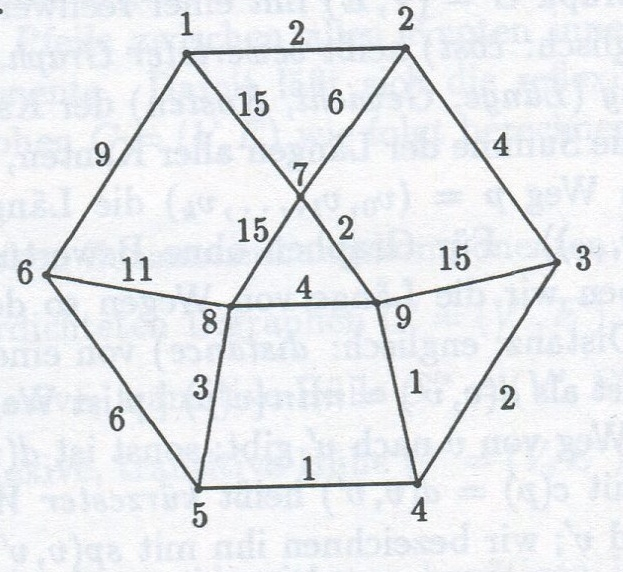
\includegraphics[width = 8cm]{./pictures/Graph.jpg}
\caption{Beispielgraph %\cite[S.572 Abb. 8.18]{OttWid90}
%{\tiny (Quelle: OTTMANN, Thomas; WIDMAYER Peter: Algorithmen und Datenstrukturen, Reihe Informatik Bd. 70, Mannheim: BI-Wissenschaftsverlag, 1990, S.572 Abb. 8.18)} 
}
\label{a1}
\end{figure}
\end{frame}
	